\chapter{Installation on Windows platform}\label{sec:WinInstall}


\paragraph{}The FA$\mu$ST project is based on \textbf{C++ library} available for Linux, MAC OS X and Windows platforms. The proposed toolbox provides a Matlab wrapper. \textbf{CMake} has been chosen to build the project FA$\mu$ST because it is an open-source, cross-platform family of tools designed to build, test and package software. This chapter presents the steps to install the FA$\mu$ST tools on Windows platform.

\begin{itemize}
\item Firstly, please ensure that the \textbf{prerequisites components} listed in Section \ref{sec:WinRequired} are installed. 

\item Secondly, \textbf{choose your preferred compiler} between GCC from MinGW "Minimalist GNU for Windows"(Section \ref{sec:WinInstallMinGW}) or from Microsoft Visual Studio (Section \ref{sec:WinInstallVS}. 

\item Then, \textbf{process to Basic installation} of FA$\mu$ST tool by following instructions given in the appropriate section, depending to the kind of compiler (MinGW or Microsoft Visual) and the use (or not) of an IDE (Integrated Development Environment). 
\end{itemize}


%Then refer to the appropriate section : If you are more familiar with the graphical user interface, prefer the basic installation using \textbf{"the IDE Visual Studio"}. Otherwise, if you are friendly with Unix tools and command line terminal, prefer the basic installation using \textbf{the command terminal}: 


Section \ref{sec:WinCustomInstall} describes the configure options available to build the FA$\mu$ST toolbox, to propose an Custom - Advanced installation. For example, the optional configuration can be used to modify the install directory path, or to build in debug mode.  


\section{Required components}\label{sec:WinRequired}
The installation of the FA$\mu$ST tool depends on other components to be installed in order to run properly. 

\begin{itemize}
\item \textbf{Install CMake}: Download Binary distributions correspond to your environment from \url{https://cmake.org/download/}.
\item \textbf{Verify CMake install} : Open a terminal and type the following command:
\begin{lstlisting}
> where cmake
\end{lstlisting}
You should obtain the path of your \texttt{cmake.exe} binary file. If not, verify that the CMAKE install directory is without any space character. Otherwise, please add the directory of your \texttt{cmake.exe} file in your environment variable. (to add an environment variable, follow instructions given in \ref{sec:ANNEXEEnvironmentVariableWindows}). 

\item \textbf{Install Matlab} (\url{https://fr.mathworks.com/downloads/}). You must install Matlab in the default directory like:
%\lstset{backgroundcolor=\color{white}}
\begin{lstlisting}[backgroundcolor=\color{white}] 
C:\Program Files\MATLAB
C:\Program Files (x86)\MATLAB
\end{lstlisting}
or install Matlab in a directory without any space character.

\item \textbf{Verify Matlab install} by checking the \texttt{matlab.exe} binary file in the default directory, for example in  
\begin{lstlisting}[backgroundcolor=\color{white}]
C:\Program Files\MATLAB\<R2015b>\bin\matlab.exe
\end{lstlisting}
In the case of an installation in a directory without any space character, type in a terminal the following command : 
\begin{lstlisting}
> where matlab
\end{lstlisting}
You must obtain the path of your matlab binary file like: 
\begin{lstlisting}[backgroundcolor=\color{white}]
C:\ProgramFiles\MATLAB\<R2015b>\bin\matlab.exe
\end{lstlisting}
If not, please add the directory of your \texttt{matlab.exe} file in your environment variable. (to add an environment variable, follow instructions given in \ref{sec:ANNEXEEnvironmentVariableWindows}). 


\item \textbf{Install 7-zip tool} from \url{http://www.7-zip.org/} in a install directory without any space character. 
\item \textbf{Verify 7-zip install} by typing in a terminal the following command : 
\begin{lstlisting}
> where 7z
\end{lstlisting}
You must obtain the path of your \texttt{7z.exe} binary file: 
\begin{lstlisting}[backgroundcolor=\color{white}]
C:\program\7-Zip\7z.exe
\end{lstlisting}
If not, verify that the 7-Zip install directory is without any space character. Otherwise, add \texttt{7z.exe} directory in your environment path. 
(to add an environment variable, follow instructions given in \ref{sec:ANNEXEEnvironmentVariableWindows}). 

\end{itemize}

\section{Download Faust Package}\label{sec:WinDownload}
When prerequisities listed in precedent section \ref{sec:WinRequired} are checked, you can get the package FA$\mu$ST.
\begin{itemize}
\item \textbf{Download} the FA$\mu$ST package on the website :  \url{http://faust.gforge.inria.fr/}
\item \textbf{Unzip} the FA$\mu$ST package into your FA$\mu$ST directory. 
\begin{lstlisting}
> 7z x FAUST-Source-2.0.0.zip
\end{lstlisting}
\end{itemize}



\section{Install using GCC-MinGW compiler}\label{sec:WinInstallMinGW}

\paragraph{}When prerequisites listed in previous section \ref{sec:WinRequired} are checked, you must install \textbf{MinGW containing the C++ Compiler}. 
Then, the FA$\mu$ST installation can be done using Command prompt, following instructions given in Section \ref{sec:WinMinGWBasicInstall} or using CodeBlocks IDE, following instructions given in Section \ref{sec:WinCodeBlocksBasicInstall}. 


\subsection{Install GCC from MinGW}
\label{sec:WinInstallCompilerMinGW}

\begin{itemize}
\item \textbf{Download MinGW} in \url{https://sourceforge.net/projects/mingw/files/latest/download?source=files}
\item \textbf{Launch install file} and choose MinGW version 4.9.2 for mex tool compatibility. The install directory must be \textbf{without any space character}.  
\item Add \texttt{gcc.exe} directory in your environment path. 
(to add an environment variable, follow instructions given in \ref{sec:ANNEXEEnvironmentVariableWindows}). 
\item \textbf{Verify MinGW install} by typing in a terminal the following command : 
\begin{lstlisting}
> where gcc
\end{lstlisting}
You must obtain the path of your \texttt{gcc.exe} binary file: 
\begin{lstlisting}[backgroundcolor=\color{white}]
C:\mingw-w64\mingw64\bin\gcc.exe
\end{lstlisting}
If not, add \texttt{gcc.exe} directory in your environment path. 
(to add an environment variable, follow instructions given in \ref{sec:ANNEXEEnvironmentVariableWindows}). 

\item \textbf{Verify make tool:} In a terminal command, type
\begin{lstlisting}
> where make
\end{lstlisting}
You must obtain the path of your \texttt{make.exe} binary file. 
If not, verify that the MINGW install directory is without any space character. Otherwise, please check if \texttt{make.exe} file is present in MINGW install directory. If not, you can copy and rename \texttt{mingw32-make.exe} to \texttt{make.exe}.

\item From Matlab IDE, you must install MinGW version 4.9.2 using the \textbf{ADDON menu}. For more detail, please follow the instruction given in following link :  
\url{http://fr.mathworks.com/help/matlab/matlab_external/install-mingw-support-package.html}. For that, you must have a id session for Mathwork (easy to create). Current this latest step, an environment variable called MW\_MINGW64\_LOC is automatically generated. 
\end{itemize}


\subsection{Basic Build \& Install using the command prompt}
\label{sec:WinMinGWBasicInstall}

The basic install described in this section requires the GCC compiler from MinGW (see precedent Section \ref{sec:WinInstallCompilerMinGW}).
If you have administrator privilege, follow instructions in Section \ref{sec:WinMinGWadminBasicInstall}, otherwise follow instructions given in Section \ref{sec:WinMinGWNoAdminBasicInstall}.
\subsubsection{Install with administrator privilege}
\label{sec:WinMinGWadminBasicInstall}

\begin{itemize}
\item Open a command terminal
\item Set the current directory to your FA$\mu$ST directory (NOTE: don't use any special character in your FAUST directory path, for example the character $\mu$)
\item Type the following commands : 
\begin{lstlisting}
> mkdir build
> cd build
> cmake -G "MinGW Makefiles" .. 
> make
\end{lstlisting}

\item Open a command terminal \textbf{with administrator privilege} : right click on command prompt icon and select run as administrator. 
\item Set the current directory to your FA$\mu$ST directory
\item Type the following commands : 
\begin{lstlisting}
> make install 
\end{lstlisting}
\end{itemize}

\subsubsection{Install without administrator privilege}
\label{sec:WinMinGWNoAdminBasicInstall}

\begin{itemize}
\item Open a command terminal
\item Set the current directory to your FA$\mu$ST directory (NOTE: don't use any special character in your FAUST directory path, for example the character $\mu$)
\item Type the following commands : 
\begin{lstlisting}
> mkdir build
> cd build
> cmake -G "MinGW Makefiles" .. 
	    -DCMAKE\_INSTALL\_PREFIX="<Your/Install/Dir>"
> make
> make install 
\end{lstlisting}
\end{itemize}


\subsection{Basic build \& Install using Code::Blocks IDE}
\label{sec:WinCodeBlocksBasicInstall}

The basic install described in this section requires the GCC compiler from MinGW (see precedent Section \ref{sec:WinInstallCompilerMinGW}).
If you have administrator privilege, follow instructions in Section \ref{sec:WinMinGWCodeBlocksAdminBasicInstall}, otherwise follow instructions given in Section \ref{sec:WinMinGWCodeBlocksNoAdminBasicInstall}.

You must select the gcc compiler in the IDE code::Blocks in the \\ \texttt{Settings menu --> Compiler... --> Selected Compiler }  

Then, the FA$\mu$ST installation can be done. 

\subsubsection{Install with administrator privilege}
\label{sec:WinMinGWCodeBlocksAdminBasicInstall}
\begin{itemize}
\item Open a command terminal
\item Set the current directory to your FA$\mu$ST directory (NOTE: don't use any special character in your FAUST directory path, for example the character $\mu$)
\item Type the following commands : 
\begin{lstlisting}
> mkdir build
> cd build
> cmake -G "CodeBlocks - MinGW Makefiles" .. 
\end{lstlisting}
\item Open the FA$\mu$ST project from the file \texttt{./build/FAUST.cbp} with Code::Blocks IDE.
\item In Code::Blocks IDE, select ALL target and build the project.
\item Re-Open the FA$\mu$ST project from the file ./build/FAUST.cbp with Code::Blocks IDE \textbf{with administrator privilege}. For that, right-click on the Code::Blocks icon and select "run as administrator". 
\item In Code::Blocks IDE, select INSTALL target and build the project.
For more detail about cmake commands, refer to Section \ref{sec:ANNEXEInfoBuildInstall}.
\end{itemize}

\subsubsection{Install without administrator privilege}
\label{sec:WinMinGWCodeBlocksNoAdminBasicInstall}
\begin{itemize}
\item Open a command terminal
\item Set the current directory to your FA$\mu$ST directory (NOTE: don't use any special character in your FAUST directory path, for example the character $\mu$)
\item Type the following commands : 
\begin{lstlisting}
> mkdir build
> cd build
> cmake -G "CodeBlocks - MinGW Makefiles" .. 
	    -DCMAKE\_INSTALL\_PREFIX="<Your/Install/Dir>"
\end{lstlisting}
\item Open the FA$\mu$ST project from the file \texttt{./build/FAUST.cbp} with Code::Blocks IDE.
\item In Code::Blocks IDE, select ALL target and build the project.
\item In Code::Blocks IDE, select install target and build the project.
For more detail about cmake commands, refer to Section \ref{sec:ANNEXEInfoBuildInstall}.
\end{itemize}





% MICCORSOFT VISUAL STUDIO
\section{Install using Microsoft Visual compiler}\label{sec:WinInstallVS}

\paragraph{}When prerequisites listed in section \ref{sec:WinRequired} are checked, you must install \textbf{Microsoft Visual Studio} containing the C++ Compiler (Section \ref{sec:WinInstallCompilerVS}).
Then, the FA$\mu$ST installation can be done using Visual Studio IDE, following instructions given in Section \ref{sec:WinVisualStudioBasicInstall} or using Command prompt, following instructions given in Section \ref{sec:WinVisualStudioTerminalBasicInstall}. 


%If you are more familiar with the graphical user interface, prefer the \textbf{Microsoft Visual C++} compiler. Otherwise, if you are friendly with Unix tools and command line terminal, preferd \textbf{MinGW "Minimalist GNU for Windows"} C++ compiler. The version of the C++ compiler must be coherent with the version of your Matlab version. In this documentation, the version of our C++ compiler corresponds to Matlab 2014 and 2015. If you use an other version of Matlab, please refer to the Mathworks website \url{http://fr.mathworks.com/support/compilers/<R20XXa>}.

\subsection{Install Microsoft Visual compiler}\label{sec:WinInstallCompilerVS} 

\begin{itemize}
\item Download Microsoft Visual Studio Professional 2013 from \url{https://www.microsoft.com/en-US/download/details.aspx?id=44916}
\item Install Microsoft Visual Studio Professional 2013
% \item Download and install Microsoft .NET Framework 4
% \item Download and install Microsoft SDK 7.1
\end{itemize}
Then, the FA$\mu$ST installation can be done using Visual Studio IDE, following instructions given in Section \ref{sec:WinVisualStudioBasicInstall} or using Command prompt, following instructions given in Section \ref{sec:WinVisualStudioTerminalBasicInstall}. 

\subsection{Basic Build \& Install using Visual Studio IDE}\label{sec:WinVisualStudioBasicInstall}
The basic install described in this section requires Microsoft Visual Studio (see precedent Section \ref{sec:WinInstallCompilerVS}).
If you have administrator privilege, follow instructions in Section \ref{sec:AdminWinVisualStudioBasicInstall}, otherwise follow instructions given in Section \ref{sec:NoAdminWinVisualStudioBasicInstall}.

\subsubsection{Install with administrator privilege}
\label{sec:AdminWinVisualStudioBasicInstall}
\begin{itemize}
\item Open a command terminal
\item Set the current directory to your FA$\mu$ST directory (NOTE: don't use any special character in your FAUST directory path, for example the character $\mu$)
\item Type the following commands : 
\begin{lstlisting}
> mkdir build
> cd build
> cmake .. 
\end{lstlisting}
\item Open the FA$\mu$ST project from the file \texttt{./build/FAUST.sln} with Visual Studio IDE.
\item In Visual Studio IDE, select ALL target and generate the project three times.
\item Re-Open the FA$\mu$ST project from the file \texttt{./build/FAUST.sln} with Visual Studio IDE with \textbf{administrator privilege}.
\item In Visual Studio IDE, select install target and generate the project.
For more detail about cmake commands, refer to Section \ref{sec:ANNEXEInfoBuildInstall}.
\end{itemize}

 
\subsubsection{Install without administrator privilege}
\label{sec:NoAdminWinVisualStudioBasicInstall}

\begin{itemize}

\item Open a command terminal
\item Set the current directory to your FA$\mu$ST directory (NOTE: don't use any special character in your FAUST directory path, for example the character $\mu$)
\item Type the following commands : 
\begin{lstlisting}
> mkdir build
> cd build
> cmake .. -DCMAKE\_INSTALL\_PREFIX="<Your/Install/Dir>"
\end{lstlisting}
\item Open the FA$\mu$ST project from the file \texttt{./build/FAUST.sln} with Visual Studio IDE.
\item In Visual Studio IDE, select ALL target and generate the project three times.
\item In Visual Studio IDE, select install target and generate the project.
For more detail about cmake commands, refer to Section \ref{sec:ANNEXEInfoBuildInstall}.

\end{itemize}

\subsection{Basic Build \& Install using terminal}\label{sec:WinVisualStudioTerminalBasicInstall}
The basic install described in this section requires the Microsoft Visual Studio compiler (see precedent Section \ref{sec:WinInstallCompilerVS}).
If you have administrator privilege, follow instructions in Section \ref{sec:AdminWinVisualStudioTerminalBasicInstall}, otherwise follow instructions given in Section \ref{sec:NoAdminWinVisualStudioTerminalBasicInstall}.

\subsubsection{Install with administrator privilege}
\label{sec:AdminWinVisualStudioTerminalBasicInstall}

\begin{itemize}
\item Open a command terminal
\item Set the current directory to your FA$\mu$ST directory (NOTE: don't use any special character in your FAUST directory path, for example the character $\mu$)
\item Type the following commands : 

\begin{lstlisting}
> mkdir build
> cd build
> cmake ..
> cmake --build . --config "Release"
> cmake --build . --config "Release"
\end{lstlisting}
\item Re-Open a command terminal \textbf{with administrator privilege} 
\begin{lstlisting}
> cmake --build . --config "Release" --target "install"
\end{lstlisting}
\end{itemize}

\subsubsection{Install without administrator privilege}
\label{sec:NoAdminWinVisualStudioTerminalBasicInstall}

\paragraph{NOTE:}In the case of \textbf{Microsoft Visual Studio 2013 compiler using the command terminal} :

\begin{itemize}
\item Open a command terminal
\item Set the current directory to your FA$\mu$ST directory (NOTE: don't use any special character in your FAUST directory path, for example the character $\mu$)
\item Type the following commands : 

\begin{lstlisting}
> mkdir build
> cd build
> cmake .. -DCMAKE\_INSTALL\_PREFIX="<Your/Install/Dir>" 
> cmake --build . --config "Release"
> cmake --build . --config "Release"
> cmake --build . --config "Release" --target "install"
\end{lstlisting}
\end{itemize}






\section{Custom - Advanced Installation}\label{sec:WinCustomInstall}
\begin{enumerate}
\item Open application \texttt{cmake-GUI.exe} from the program menu or from your cmake install binaries directory  to launch the CMake configuration application:

\begin{figure}[!h] %%[!htbp]
\centering
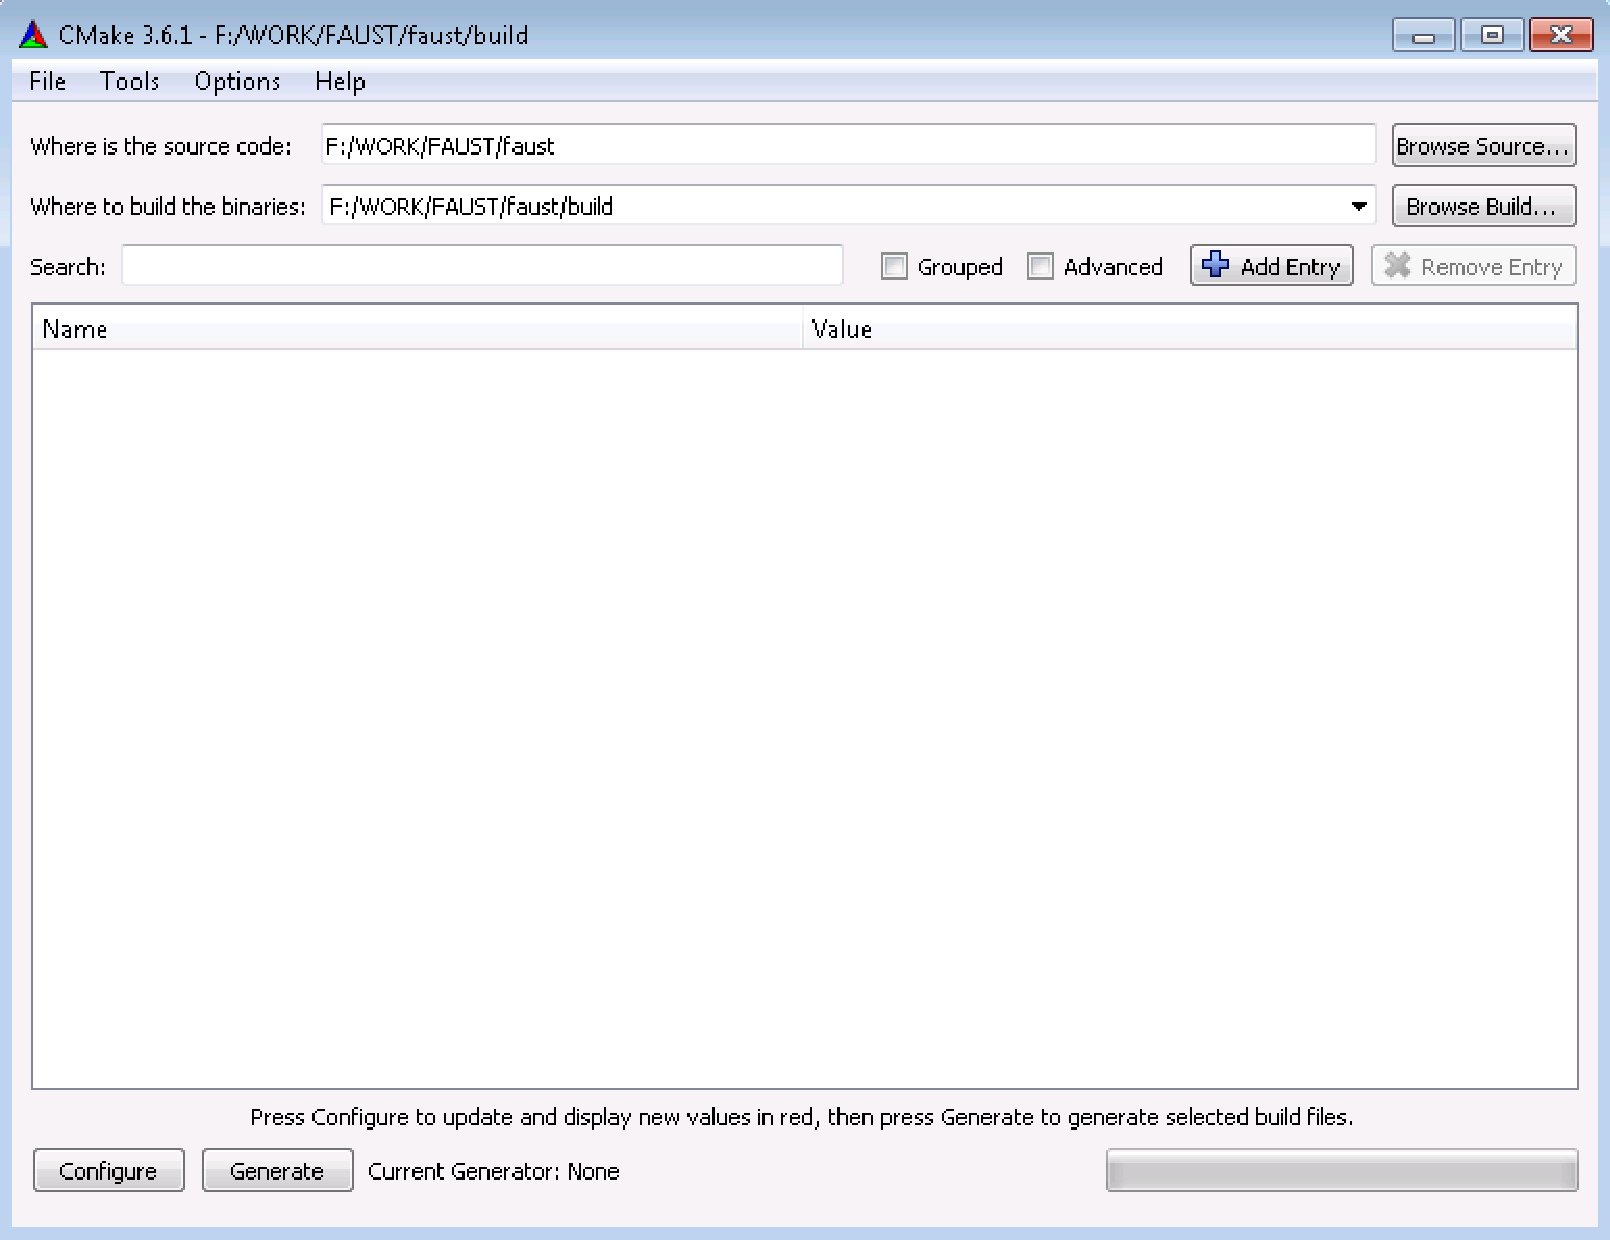
\includegraphics[scale=0.5]{images/cmakeGUI-1-eps-converted-to.pdf}
\caption{cmake GUI}
\label{fig:cmakeGUI-1}
\end{figure}

\item Set the "Where is the source code:" text box with the path of the directory where the source files are located (F:/WORK/FAUST/faust) and the "Where to build the binaries:" with the path of the directory where you want to build the library and executable files (F:/WORK/FAUST/faust/build). (see fig.  \ref{fig:cmakeGUI-1}).

When clicking for the first time on the [Configure] button, CMake will ask for the build tool you want to use. The build system type depends on the builder you want to use, in our case this is the Visual Studio X (X depending the version of Visual installed on the computer) chain tools. (see fig. \ref{fig:cmakeGUI-2}).


\begin{figure}[!h]
\centering
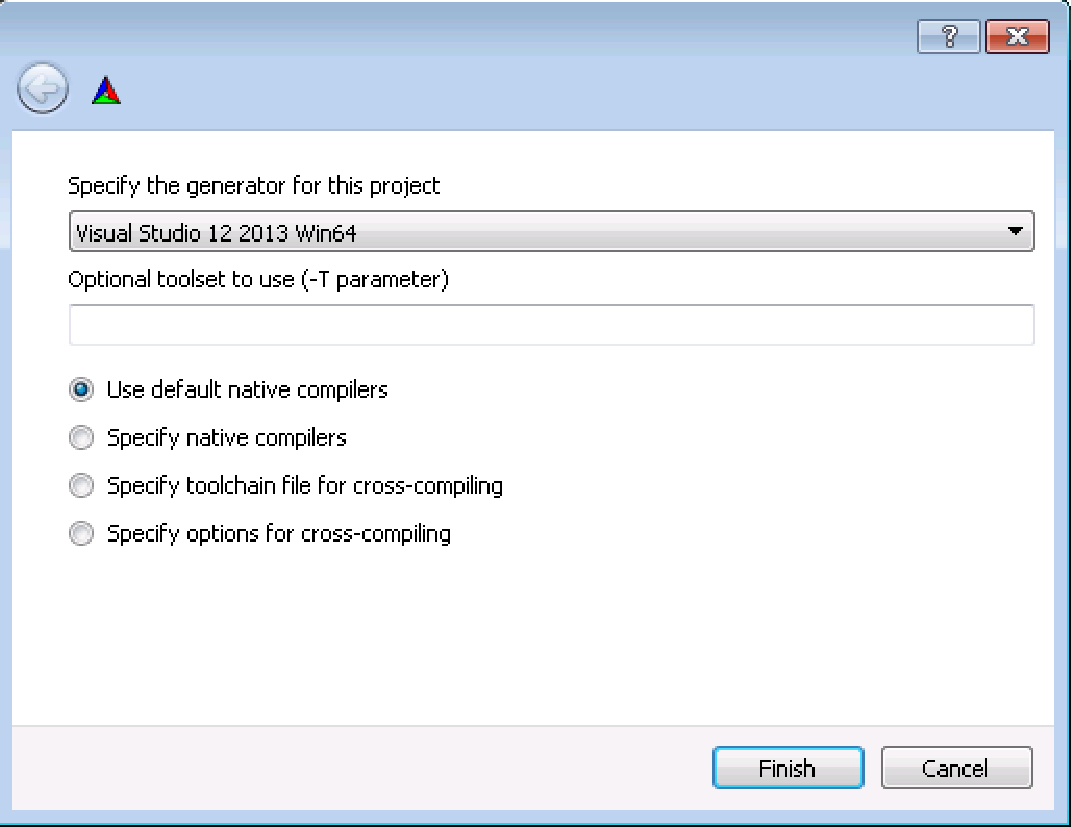
\includegraphics[scale=0.5]{images/cmakeGUI-2-eps-converted-to.pdf}
\caption{cmake GUI}
\label{fig:cmakeGUI-2}
\end{figure}

\item When pressing again the [Configure] button to configure the build system, CMake performs a list of tests to determine the system configuration and manage the build system. If the configuration is correct then no pop-up will appears during the tests and CMake finally shows the various options of the build underlaid in grey. In case of a configuration issue, a pop up window warns you about this issue indicating which test has failed, in this case the build option in the CMake application software will be underlaid in red. We will discuss in Section \ref{sec:WinCustomInstall} what to do in such a case, but let us for the moment assume that everything ran smoothly.
(see \ref{fig:cmakeGUI-4}).

\begin{figure}[!h] %%[!htbp]
\centering
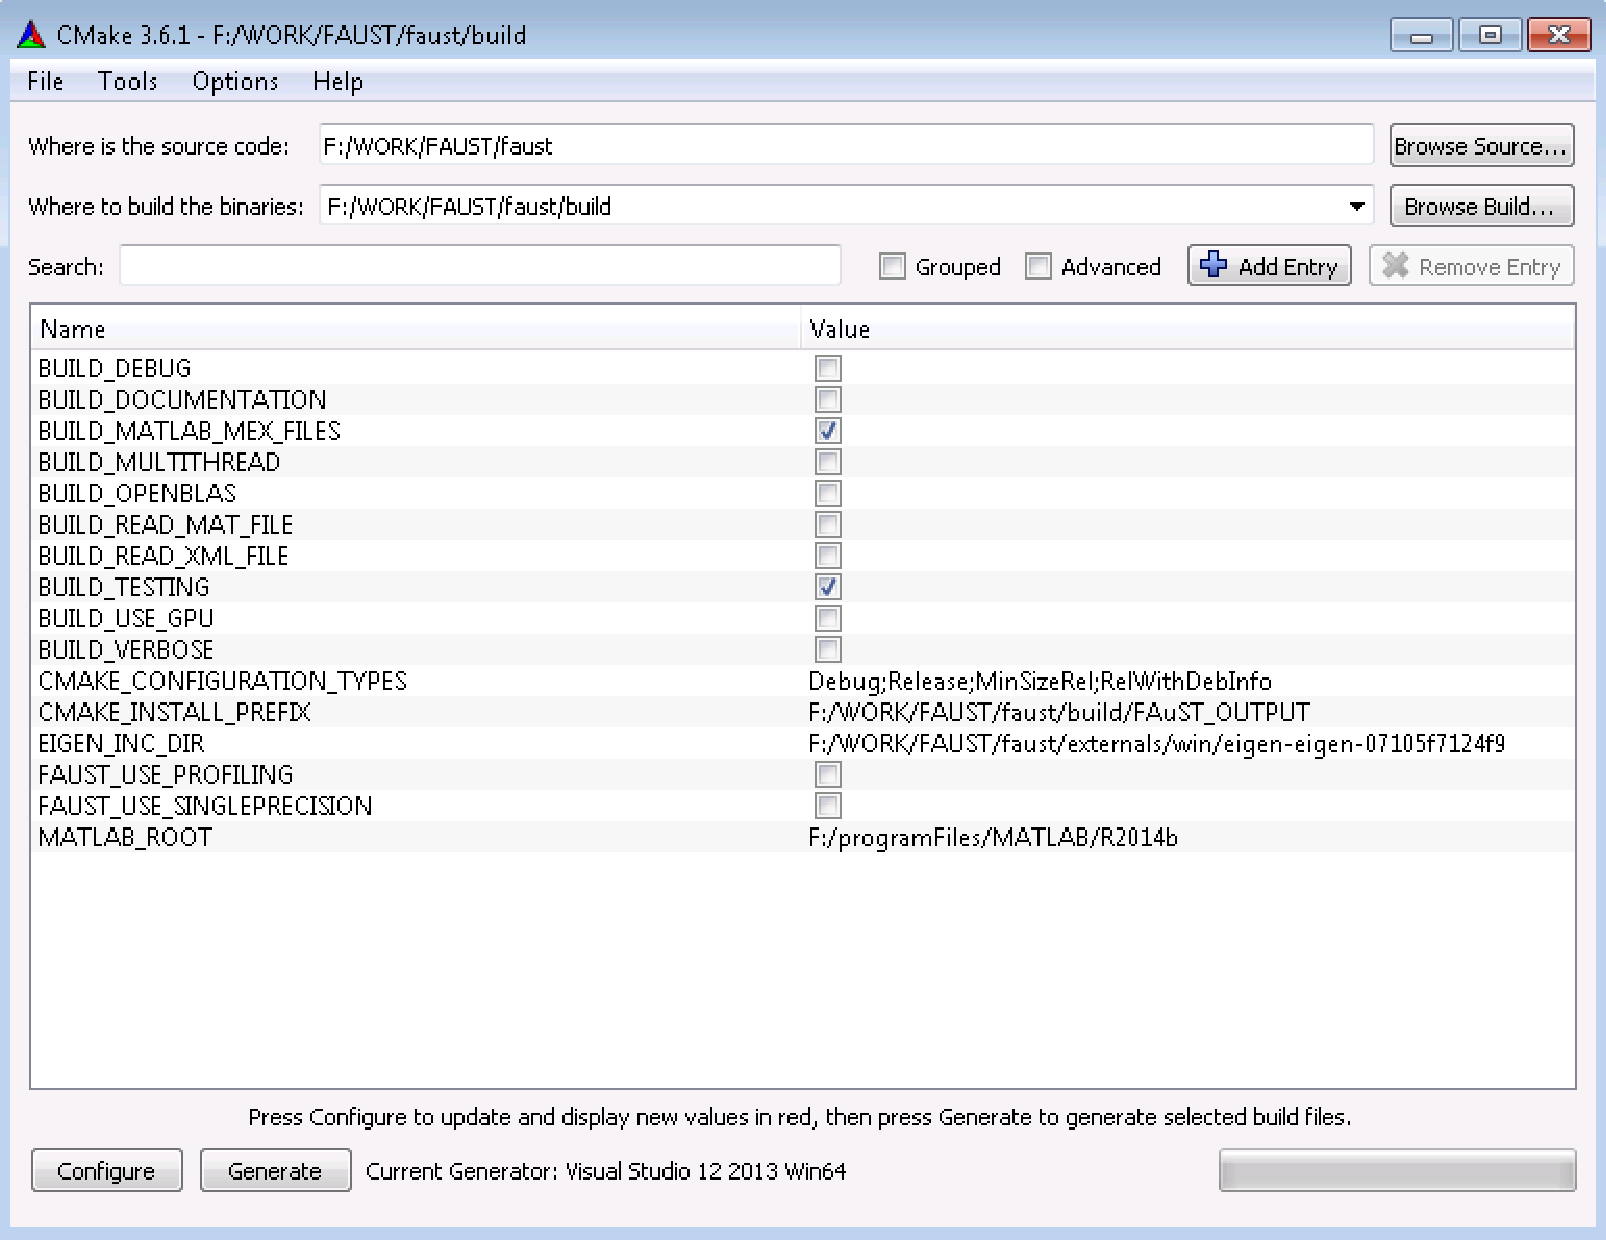
\includegraphics[scale=0.5]{images/cmakeGUI-4-eps-converted-to.pdf}
\caption{cmake GUI}
\label{fig:cmakeGUI-4}
\end{figure}

\end{enumerate}

%%%%AUTRESS


